\documentclass[17pt,titlepage,extrafontsizes]{memoir}
\usepackage[a3paper,margin=2cm,top=2.5cm]{geometry}
\usepackage{color}
\usepackage{background}
\usepackage{helvet}
\usepackage[utf8]{inputenc}
\usepackage{enumitem}
\setlist{nolistsep}
\usepackage{soul}
\setul{3pt}{2pt}
\renewcommand*{\familydefault}{\sfdefault}
\setlength{\parindent}{0pt}
\backgroundsetup{
scale=1,
angle=0,
opacity=0.4,  %% adjust
contents={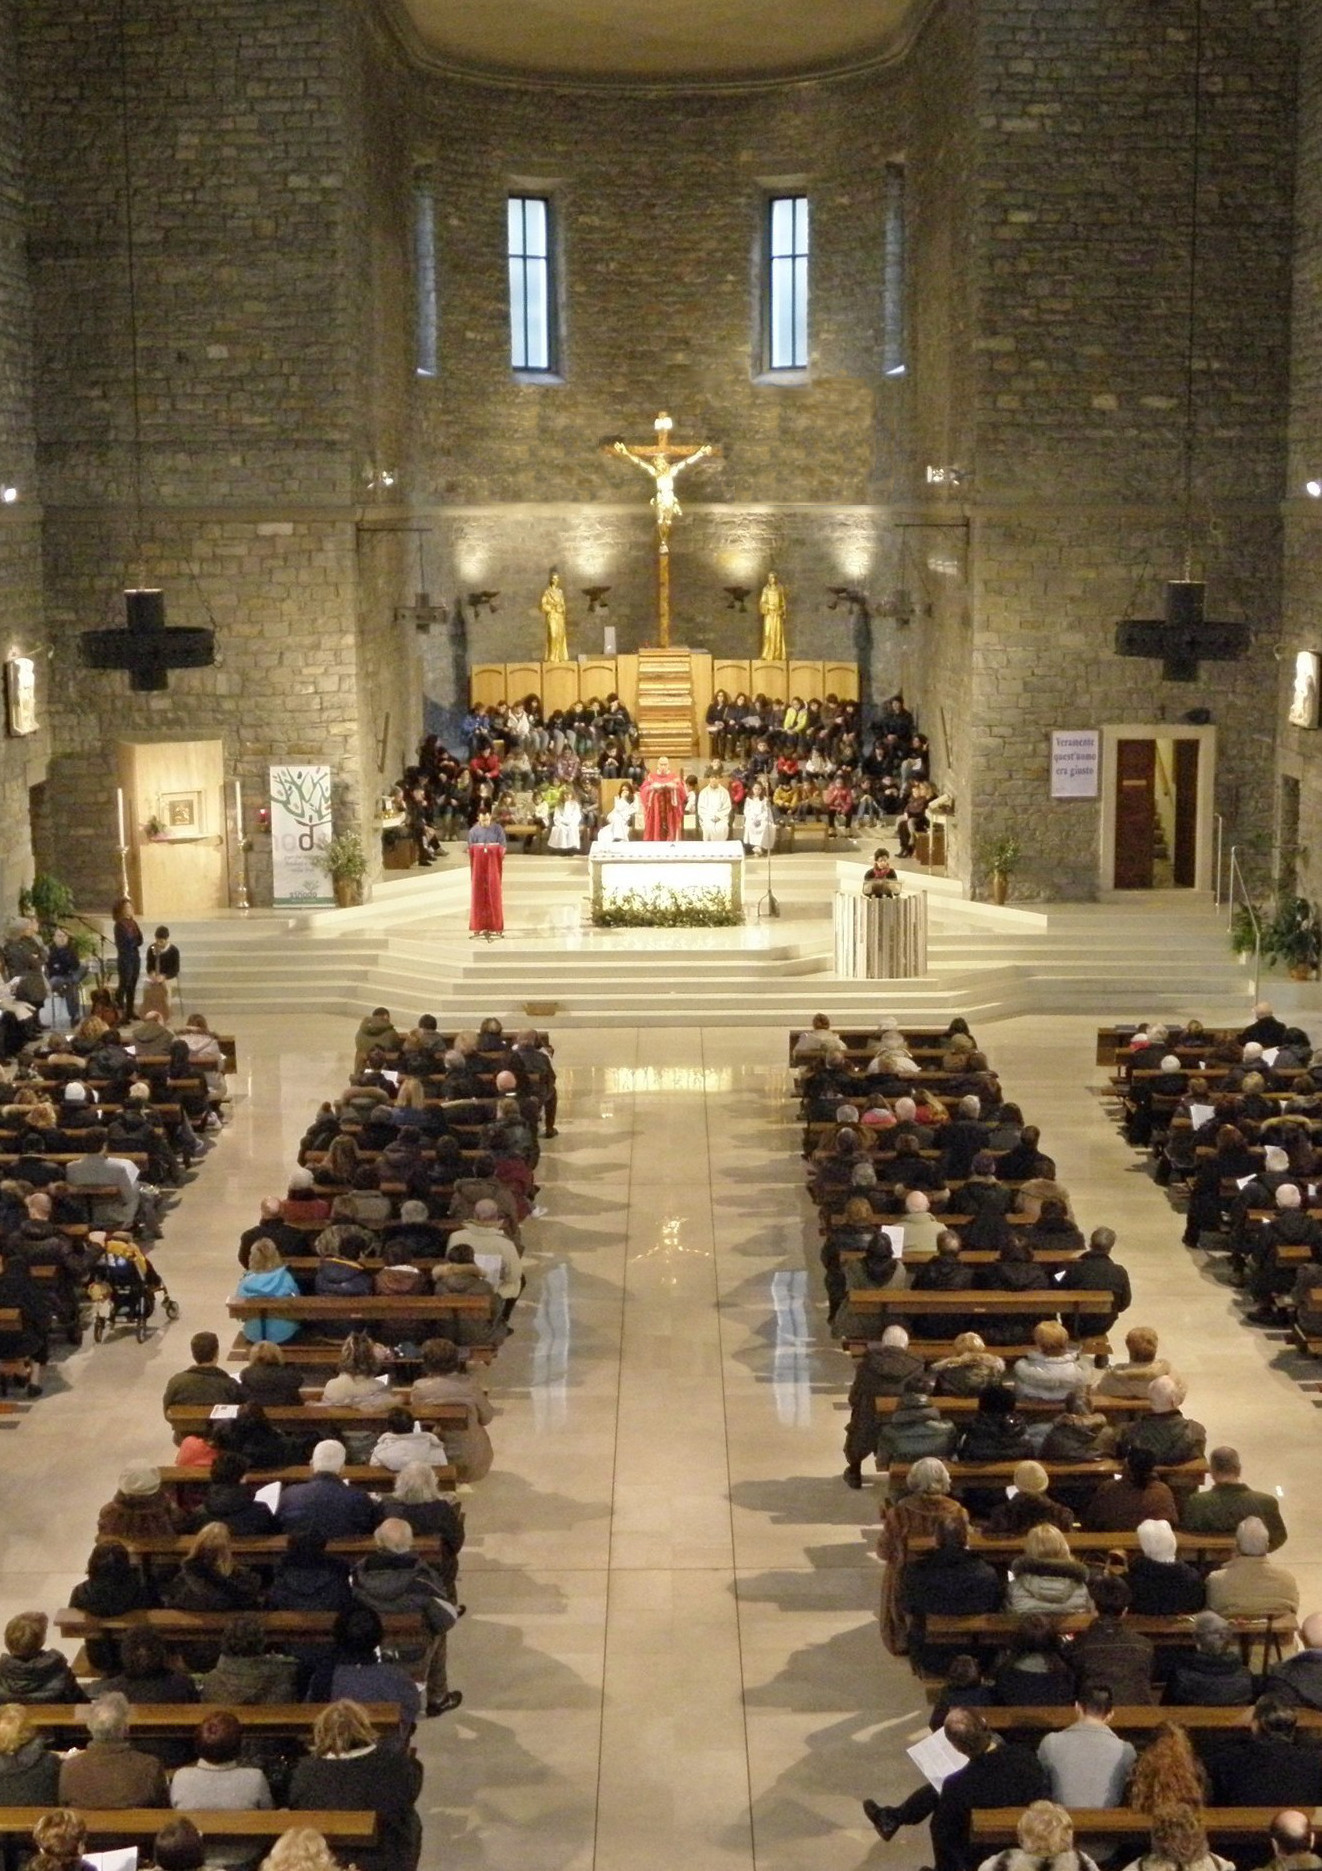
\includegraphics[width=\paperwidth,height=\paperheight ]{chiesa}}
}
\hyphenation{Giampaolo Crepaldi}
\begin{document}
\pagestyle{empty}
\begin{center}
{\LARGE PARROCCHIA di SAN FRANCESCO - TRIESTE\par
\vspace{1cm}
\textbf{1965-2015: 50 ANNI di VITA}}
\end{center}
\vfill
{\Large \ul{PROGRAMMA DELLA FESTA}:}
\par\bigskip\bigskip
\textbf{\Large DOMENICA 27 SETTEMBRE ore 20.30:}
\par\medskip
{\large Concerto del  Gruppo vocale e strumentale Soul Diesis\par}
\textit{Repertorio di brani tradizionali di ispirazione religiosa (spiritual soul e gospel).}
\par\bigskip\bigskip
\textbf{\Large LUNEDI’ 28 SETTEMBRE-DOMENICA 4 OTTOBRE:}
\par\medskip
{\large settimana di preparazione spirituale con predicazione francescana alle ss. Messe;}
\par\bigskip\bigskip
\textbf{\Large VENERDI’ 2 OTTOBRE ore 17.30-18.15:}
\par\medskip
{\large adorazione eucaristica;}
\par\bigskip\bigskip
\textbf{\Large SABATO 3 OTTOBRE}
\par\medskip
\begin{itemize}
 \large
 \item \textbf{ore 17.45:} celebrazione del \textbf{TRANSITO di san FRANCESCO} (ricordo della sua morte);
 \item \textbf{ore 18.30:} S. Messa;
 \item \textbf{ore 19.30:} Oscar A. Romero, morte per un popolo. Riduzione per una lettura drammatica e \ul{regia di Filippo Crispo}. Con la partecipazione del gruppo musicale latinoamericano \textbf{ENCUENTRO}.
\end{itemize}
\par\bigskip\bigskip
\textbf{\Large DOMENICA 4 OTTOBRE}
\par\medskip
\begin{itemize}
 \large
 \item \textbf{Ore 10.00:} S. Messa solenne presieduta dall’arcivescovo mons. Giampaolo Crepaldi, con la partecipazione delle autorità civili e religiose;
 \item \textbf{ore 12.00:} momento conviviale;
 \item \textbf{ore 16.00:} tradizionale benedizione degli animali (in porticato).
\end{itemize}
\vfill
\begin{center}
\large\bfseries 
PER L’OCCASIONE SARA’ ALLESTITA UNA PESCA di BENEFICIENZA\par
in FAVORE DEI LAVORI STRAORDINARI della PARROCCHIA:\par
\Large PER CONTINUARE PIU’ FORTI!
\end{center}
\vfill
\newpage
\end{document}